\documentclass{article}

\usepackage[utf8]{inputenc}
\usepackage[T1]{fontenc}
\usepackage[greek,english]{babel}
\usepackage{alphabeta}
\usepackage{amsmath}
\usepackage{amssymb}
\usepackage{graphicx}
\usepackage{subcaption}
\usepackage{epstopdf}
\usepackage[margin=1in, paperwidth=7.5in,paperheight=10.5in]{geometry}
\usepackage{hyperref}
\usepackage{paracol}

\newcommand\course{TΗΛ411}
\newcommand\courseName{Ψηφιακή Επεξεργασία Εικόνας}
\newcommand\semester{Χειμερινό 2021}
\newcommand\assignmentNumber{Assignment 2}
\newcommand\studentName{Μαυρογιώργης Δημήτρης}                           
\newcommand\studentNumber{2016030016}

\title{\underline{\textbf{\assignmentNumber}}} 
\author{\textsc{\textbf{Όνομα:}}  \studentName\\
		\textsc{\textbf{ΑΜ:}}  \studentNumber\\
		\course \ - \courseName\\ 
		\textsc{Πολυτεχνείο Κρήτης}
}
\date{\today}
\begin{document}
	\maketitle

\section*{Introduction}
	Ο σκοπός της 2ης εργαστηριακής άσκησης είναι να υλοποιήσουμε τη συνέλιξη μιας εικόνας με ένα Gaussian φίλτρο. Πιο συγκεκριμένα, πρέπει να υλοποιήσουμε την πράξη της συνέλιξης με τρεις διαφορετικούς τρόπους: 1) Κατασκευη μιας δικής μας συνάρτησης (convolution2D), η οποία να υλοποιεί τη συνέλιξη μια εικόνς με το φίλτρο, 2) xρήση της συνάρτησης conv2 της matlab και 3) χρήση της συνάρτησης imfilter της matlab.
		
\section*{Exercise 1 - Convolution with for loop}
	\begin{figure}[h!]
		\centering
		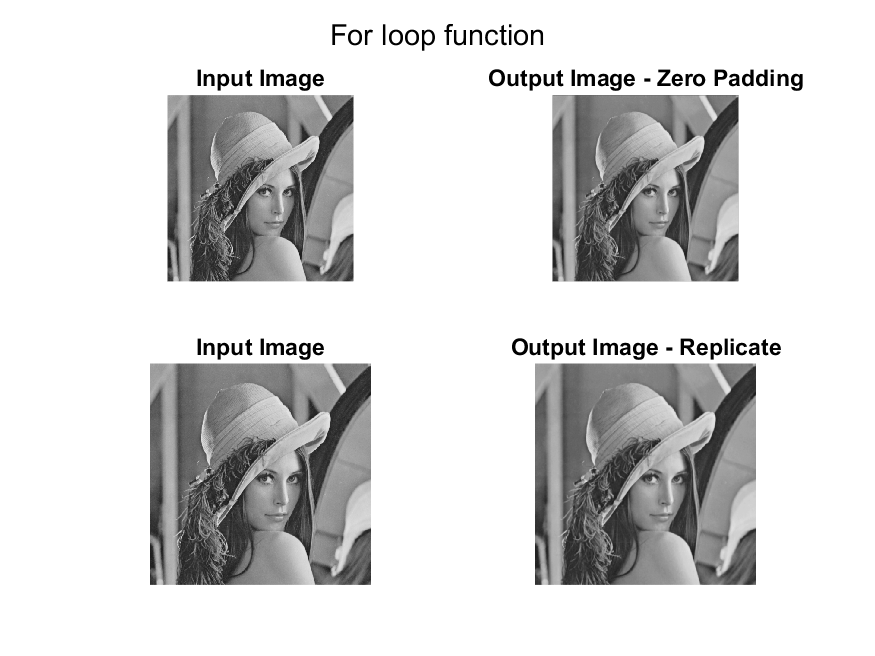
\includegraphics[width=0.8\linewidth]{./output_images/for_loop_conv.png}
		\caption{Results from my function convolution2D}
	\end{figure}
	
	\noindent
	Για την υλοποίηση της συνάρτησης convolution2D, έπρεπε να φροντίσουμε έτσι, ώστε το κεντρικό pixel του φίλτρου να ξεκινάει στο pixel (x0,y0) της εικόνας και καθώς τη διατρέχουμε να καταλήγει στο τελευταίο pixel. Γι' αυτό το λόγο, πρέπει να μεγαλώσουμε την εικόνα, ώστε το φίλτρο να μπορεί να εφαρμοστεί και στα άκρα. Για την διαδικασία αυτή, μας ζητήθηκε να προσθέσουμε μηδενικά στις γραμμές και τις στήλες ανάλογα με το μέγεθος του φίλτρου (zero padding), καθώς και να αντιγράφουμε τις γραμμεές/στήλες των άκρων (replicate). Για την συμπλήρωση των pixel χρησιμοποιήθηκε η συνάρτηση padarray, για να συμπληρώσουμε γυρω από την εικόνα μια επιπλεον σειρά από pixel.\\
	
	\noindent
	Τα αποτελέσματα των δύο μεθόδων φαίνονται στο παραπάνω figure (1). Όπως προκείπτει και από το δείκτη MSE, βλέπουμε ότι η μέθοδος replicate, βελτιώνει σε αρκετά καλό βαθμό την εικόνα. Στην περίπτωση που εφαρμόζουμε zero padding ο δείκτης MSE είναι περίπου 26.1, ενώ στην εφαρμογή της μεθόδου replicate το MSE ελαττώνεται στο 18.25.\\
	
	\noindent
	Όσον αφορά το PSNR, παρατηρούμε ότι στη περίπτωση του zero padding η τιμή του είναι 33.97, ένω στην περίπτωση του replicate η τιμή του αυξάνεται στο 35.52. Συνεπώς, βλέπουμε ότι το πηλίκο signal-to-noise ratio αυξάνεται όταν χρησιμοποιούμε τη δεύτερη μέθοδο.

\section*{Exercise 2 - Convolution with conv2 function}
	\begin{figure}[h!]
		\centering
		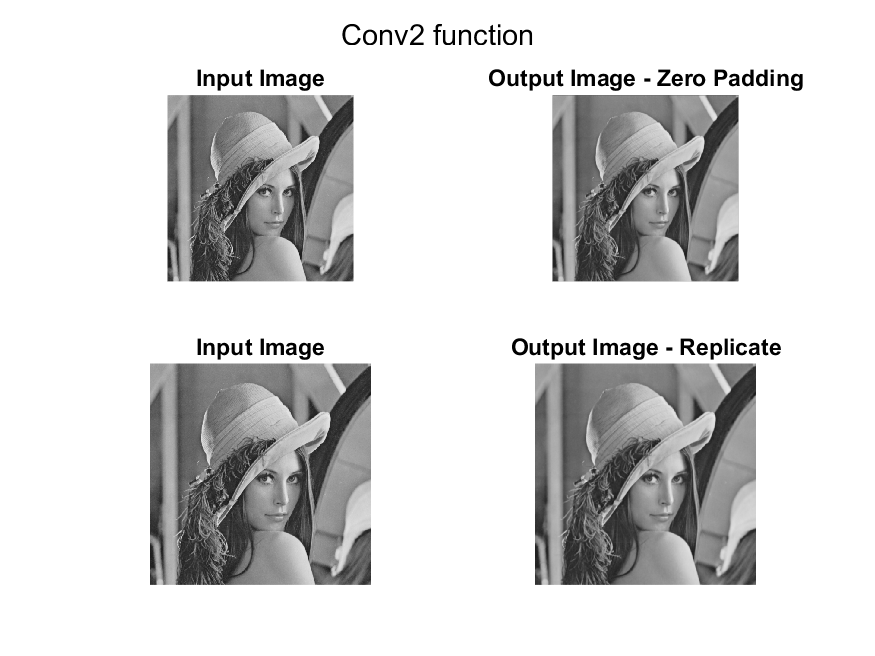
\includegraphics[width=0.8\linewidth]{./output_images/conv2_func.png}
		\caption{Results from matlab conv2 function}
	\end{figure}

	\noindent
	Σε αυτό το μέρος της άσκησης, για τη συνέλιξη της εικόνας με το φίλτρο χρησιμοποιήθηκε η συνάρτηση conv2. Για την περίπτωση του zero padding, τα ορίσματα που χρησιμοποιήθηκαν είναι η αρχική εικόνα, το φίλτρο και η παράμετρος 'same' που χρησιμοποιείται έτσι ώστε η τελική εικόνα να έχει τον ίδιο αριθμό pixel με την αρχική. Από την άλλη, στην περίπτωση του replicate, πριν εισάγουμε την εικόνα στην conv2, χρησιμοποιήθηκε η συνάρτηση padarray για να γίνει συμπλήρωση μιας επιπλέον γραμμής/στήλης γύρω από την εικόνα. Εκτός από την αρχικη εικόνα και το φίλτρο, χρησιμοποιήθηκε και η παράμετρος 'valid' έτσι, ώστε να επιστρέψουμε την εικόνα στο αρχικό της μέγεθος. \\
	
	\noindent	
	Τα αποτελέσματα των προσομοιώσεν φαίνονται στο παραπάνω figure (2). Όπως προκείπτει και από το δείκτη MSE, βλέπουμε ότι η μέθοδος replicate, βελτιώνει την εικόνα. Στην περίπτωση που εφαρμόζουμε zero padding το MSE είναι περίπου 25.2549, ενώ στην περίπτωση του replicate το MSE ελαττώνεται στο 17.2448.\\
	
	\noindent
	Όσον αφορά το PSNR, παρατηρούμε ότι στη περίπτωση του zero padding η τιμή του είναι 34.1073, ένω στην περίπτωση του replicate η τιμή του αυξάνεται στο 35.7642. Συνεπώς, βλέπουμε ότι το signal-to-noise ratio αυξάνεται, όταν χρησιμοποιούμε τη δεύτερη μέθοδο.

\section*{Exercise 3 - Convolution with imfilter function}	
	\begin{figure}[h!]
		\centering
		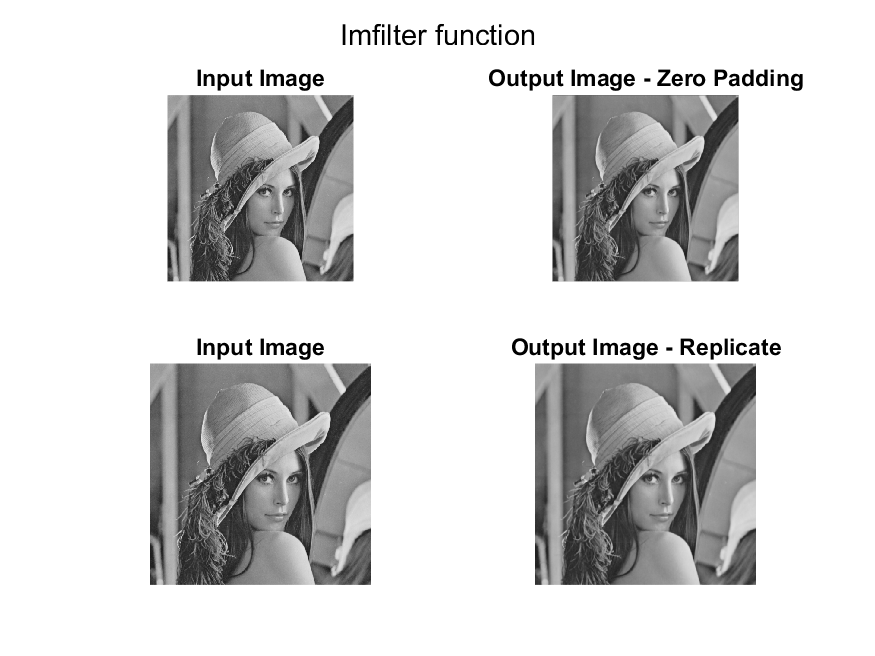
\includegraphics[width=0.8\linewidth]{./output_images/imfilter_func.png}
		\caption{Results from matlab imfilter function}
	\end{figure}
	
	\noindent
	Στο τελευταίο μέρος της άσκησης, για τη συνέλιξη έγινε χρήση της συνάρτηση imfiter. Για την περίπτωση του zero padding, οι παράμετροι που χρησιμοποιήθηκαν είναι η αρχική εικόνα, το φίλτρο και η παράμετρος 'same', για να έχουμε ίδιο μέγεθος αρχικής και τελικής εικόνας. Αντίθετα, στην περίπτωση του replicate, χρησιμοποιήθηκε μία επιπλέον παράμετρος η 'replicate'. \\
	
	\noindent
	Τα αποτελέσματα των προσομοιώσεν φαίνονται στο παραπάνω figure (3). Όπως προκείπτει από το δείκτη MSE, βλέπουμε ότι η μέθοδος replicate, βελτιώνει και σε αυτή την περίπτωση την εικόνα. Στην περίπτωση που εφαρμόζουμε zero padding το MSE είναι περίπου 25.7202, ενώ στην περίπτωση του replicate το MSE ελαττώνεται στο 17.2446.\\
	
	\noindent
	Όσον αφορά το PSNR, βλέπουμε ότι στη περίπτωση του zero padding η τιμή του είναι 34.1047, ένω στην περίπτωση του replicate η τιμή του αυξάνεται στο 35.7643. Συνεπώς, βλέπουμε ότι το signal-to-noise ratio αυξάνεται, όταν χρησιμοποιούμε τη δεύτερη μέθοδο.
\pagebreak
\section*{MSE - PSNR Results}
	Συνοψίζοντας, παρατηρούμε ότι και με τους τρεις τρόπους για συνέλιξη οι τελικές εικόνες, καθώς και οι τιμές των MSE και PSNR είναι παρόμοιες. Πιο συγκεκριμένα, για τους δείκτες MSE και PSNR βλέπουμε ότι υπάρχουν αμελητέες διαφορές μεταξύ της περίπτωσης χρήσης της conv2 και της imfilter. Επιπλέον, συγκρίνοντας τα αποτελέσματα του πρώτου μέρους με αυτά του 2ου και 3ου, οι διαφορές στις τιμές είναι μικρές, της τάξης μιας μονάδας περίπου για το MSE και περίπου 0.2 για το PSNR. Τέλος, παρακάτω παρουσιάζονται τα συγκεντρωτικά αποτελέσματα των τιμών για MSE και PSNR για όλες τις περιπτώσεις που περιγράφτηκαν παραπάνω.
	
	\begin{figure}[h!]
		\centering
		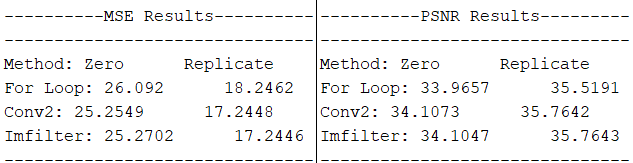
\includegraphics[width=0.8\linewidth]{./output_images/mse_psnr_results.png}
		\caption{MSE and PSNR results}
	\end{figure}
\end{document}
